\section{Caractéristiques d'un dipôle (3 points)}

Pierre a tracé le graphique caractéristique d'une résistance.

\begin{center}
	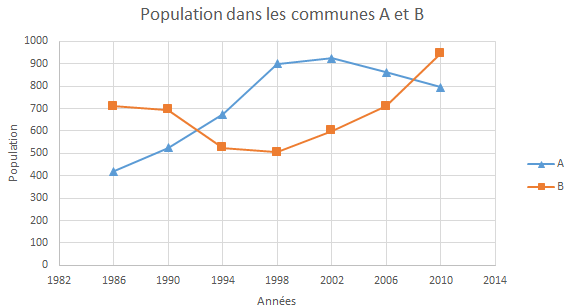
\includegraphics[scale=0.35]{img/graph}
\end{center}

\begin{questions}
	\question[1] Quelle est la tension aux bornes de la résistance lorsqu'elle est traversée par un courant d'intensité 60 $mA$ ?
	
	\question[1] Quelle est l'intensité du courant  dans la résistance si la tension à ses bornes est égale à 5 $V$ ?
	
	\question[1] Quelle est la valeur de cette résistance ?
\end{questions}